\svnid{$Id: ui.tex 248 2012-06-17 17:10:59Z dgens001 $}
\pagebreak[4]
\chapter{Benutzungsschnittstellen}

\textit{Hier findet man die Dialogspezifikation, GUI-Skizzen, die Dialogabläufe und die für das Spiel wichtige
Formatspezifikation der Campusdatei.}

\section{Ingame GUI}
Ingame gibt es vier sog. \glspl{Aktivitaetsbereich}. Im \gls{Sichtbereich} (gelb) wird dem \gls{Spieler} seine 
aktuelle Position und die angrenzenden Felder angezeigt. Zudem werden alle 
\glspl{Item} und \gls{npcs} auf dem aktuellen Feld dargestellt. Nicht begehbare Felder sind durch Wände oder
verschlossene Türen abgetrennt. Offene Türen stellen betretbare Felder dar.
\\
\begin{figure}[h]
	\begin{center}
		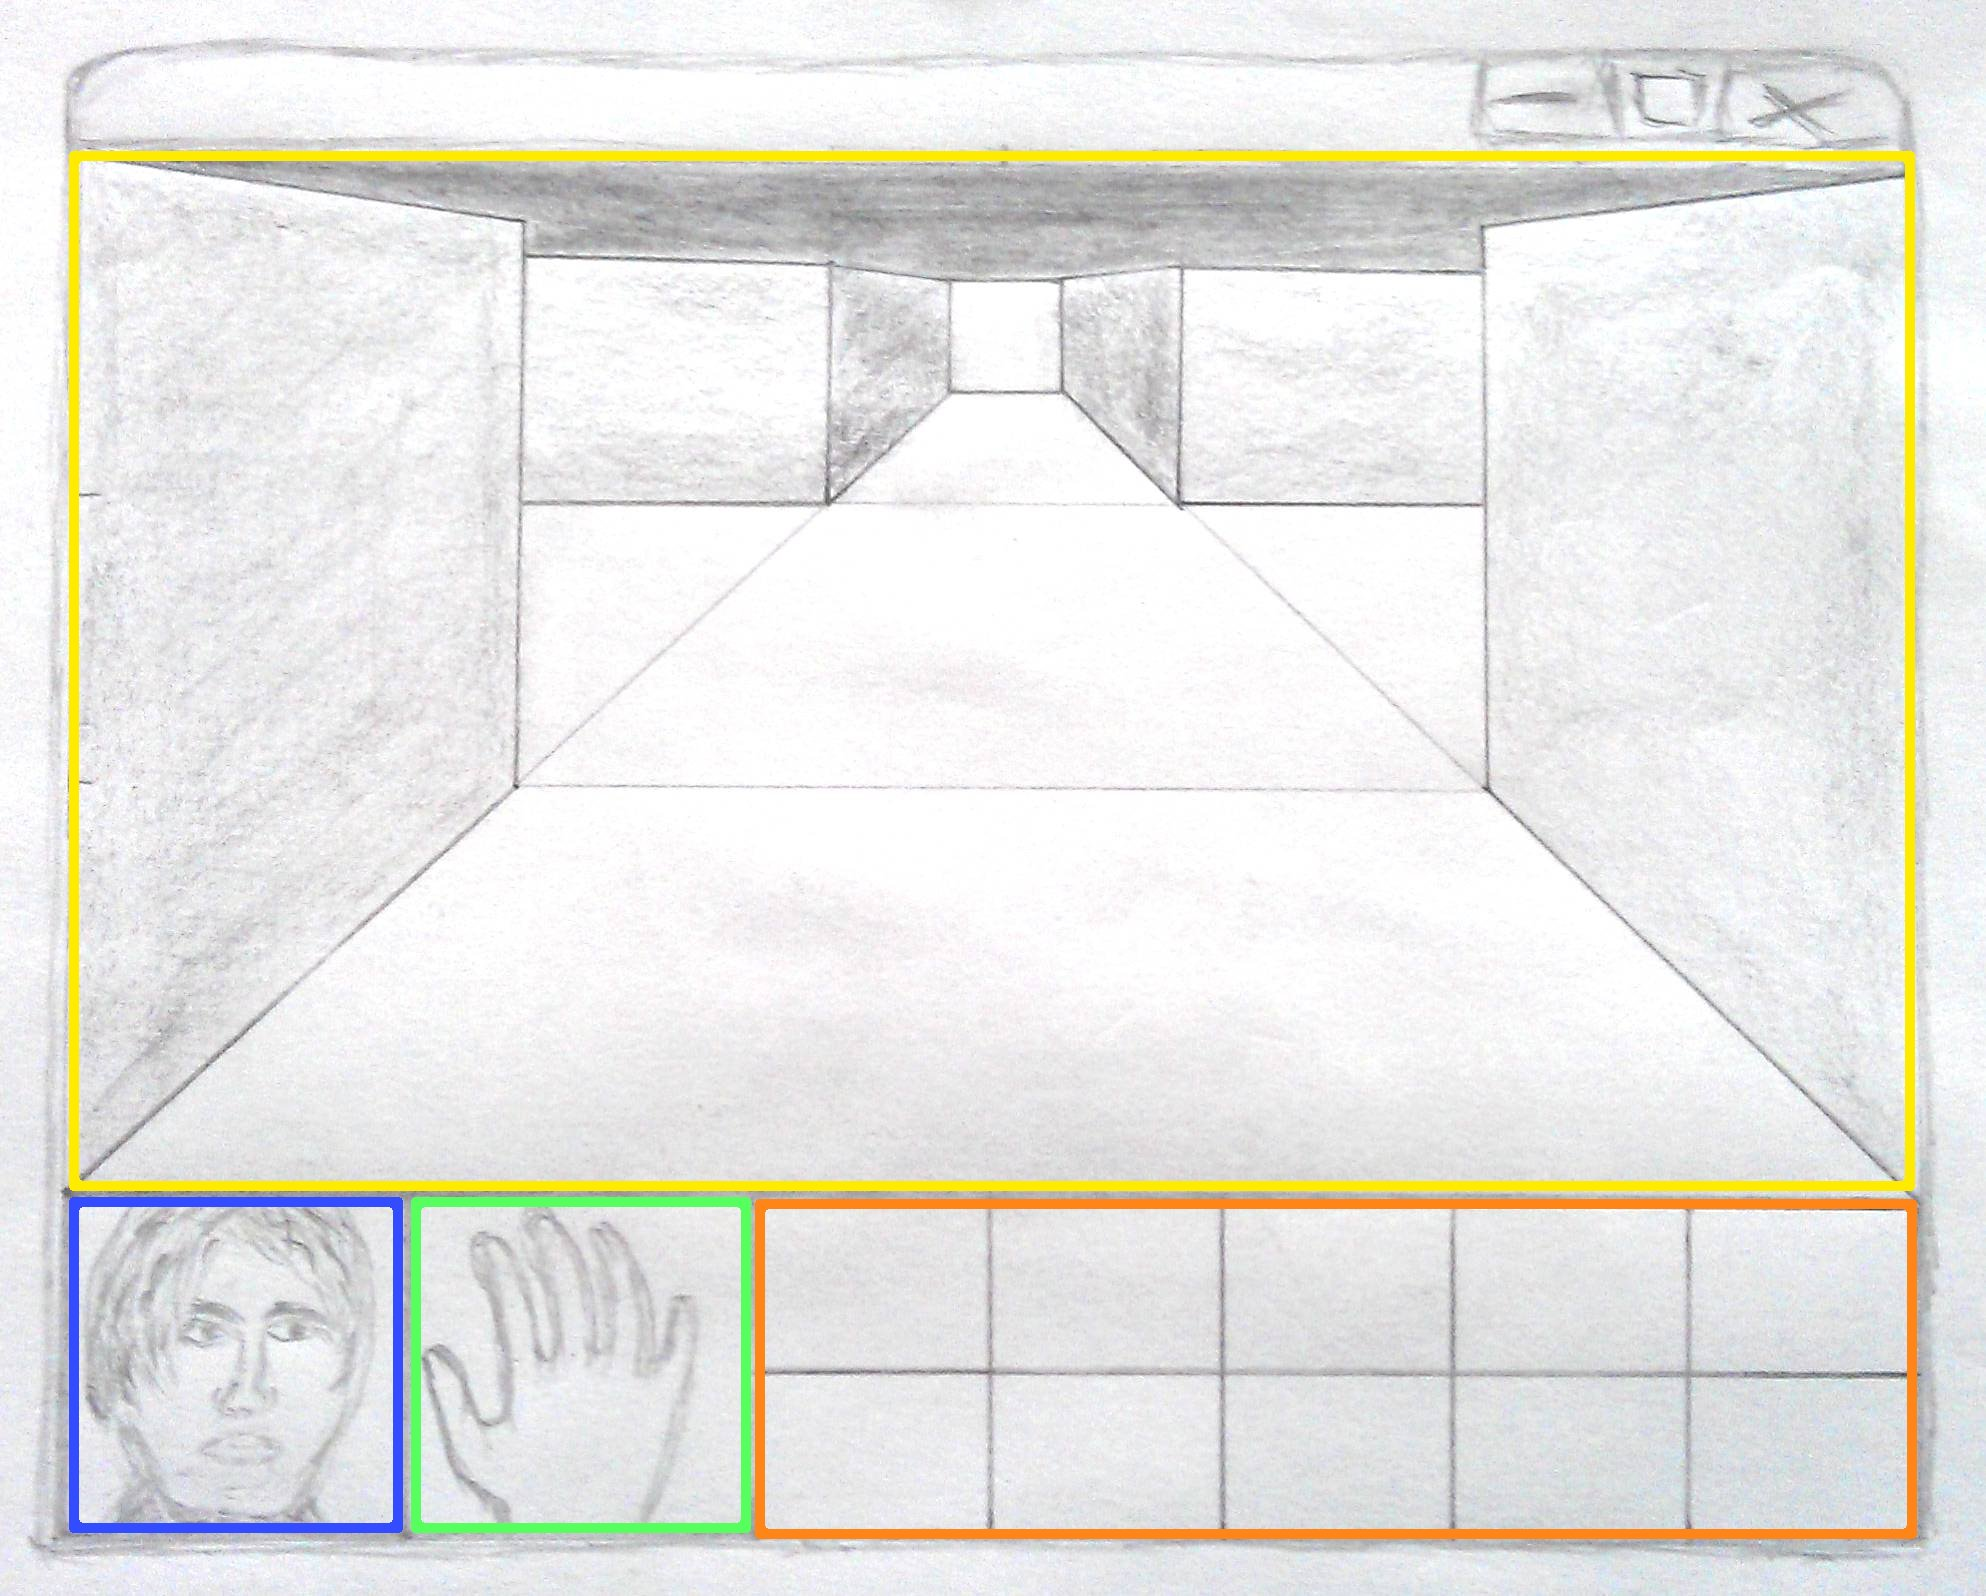
\includegraphics[width=13cm, height=10cm]{kapitel/ui/ig_kreuz_small_color.jpg}
	\end{center}
	\caption{Die vier Aktivitätsbereiche}
	\label{fig:ig_kreuz_color}
\end{figure}

Im \gls{Infobereich} (orange) hat der Spieler entweder eine Übersicht der einzelnen Inventarslots 
(Inventarsicht) oder in Interaktion textuelle Informationen (Infosicht). Der \gls{Handbereich} (grün) zeigt 
dem Spieler an, ob er ein Objekt in 
der Hand hält und falls ja, welches. Der \gls{Statusbereich} (blau) zeigt ein Porträt des Charakters.
\\
\begin{figure}[h]
	\begin{center}
		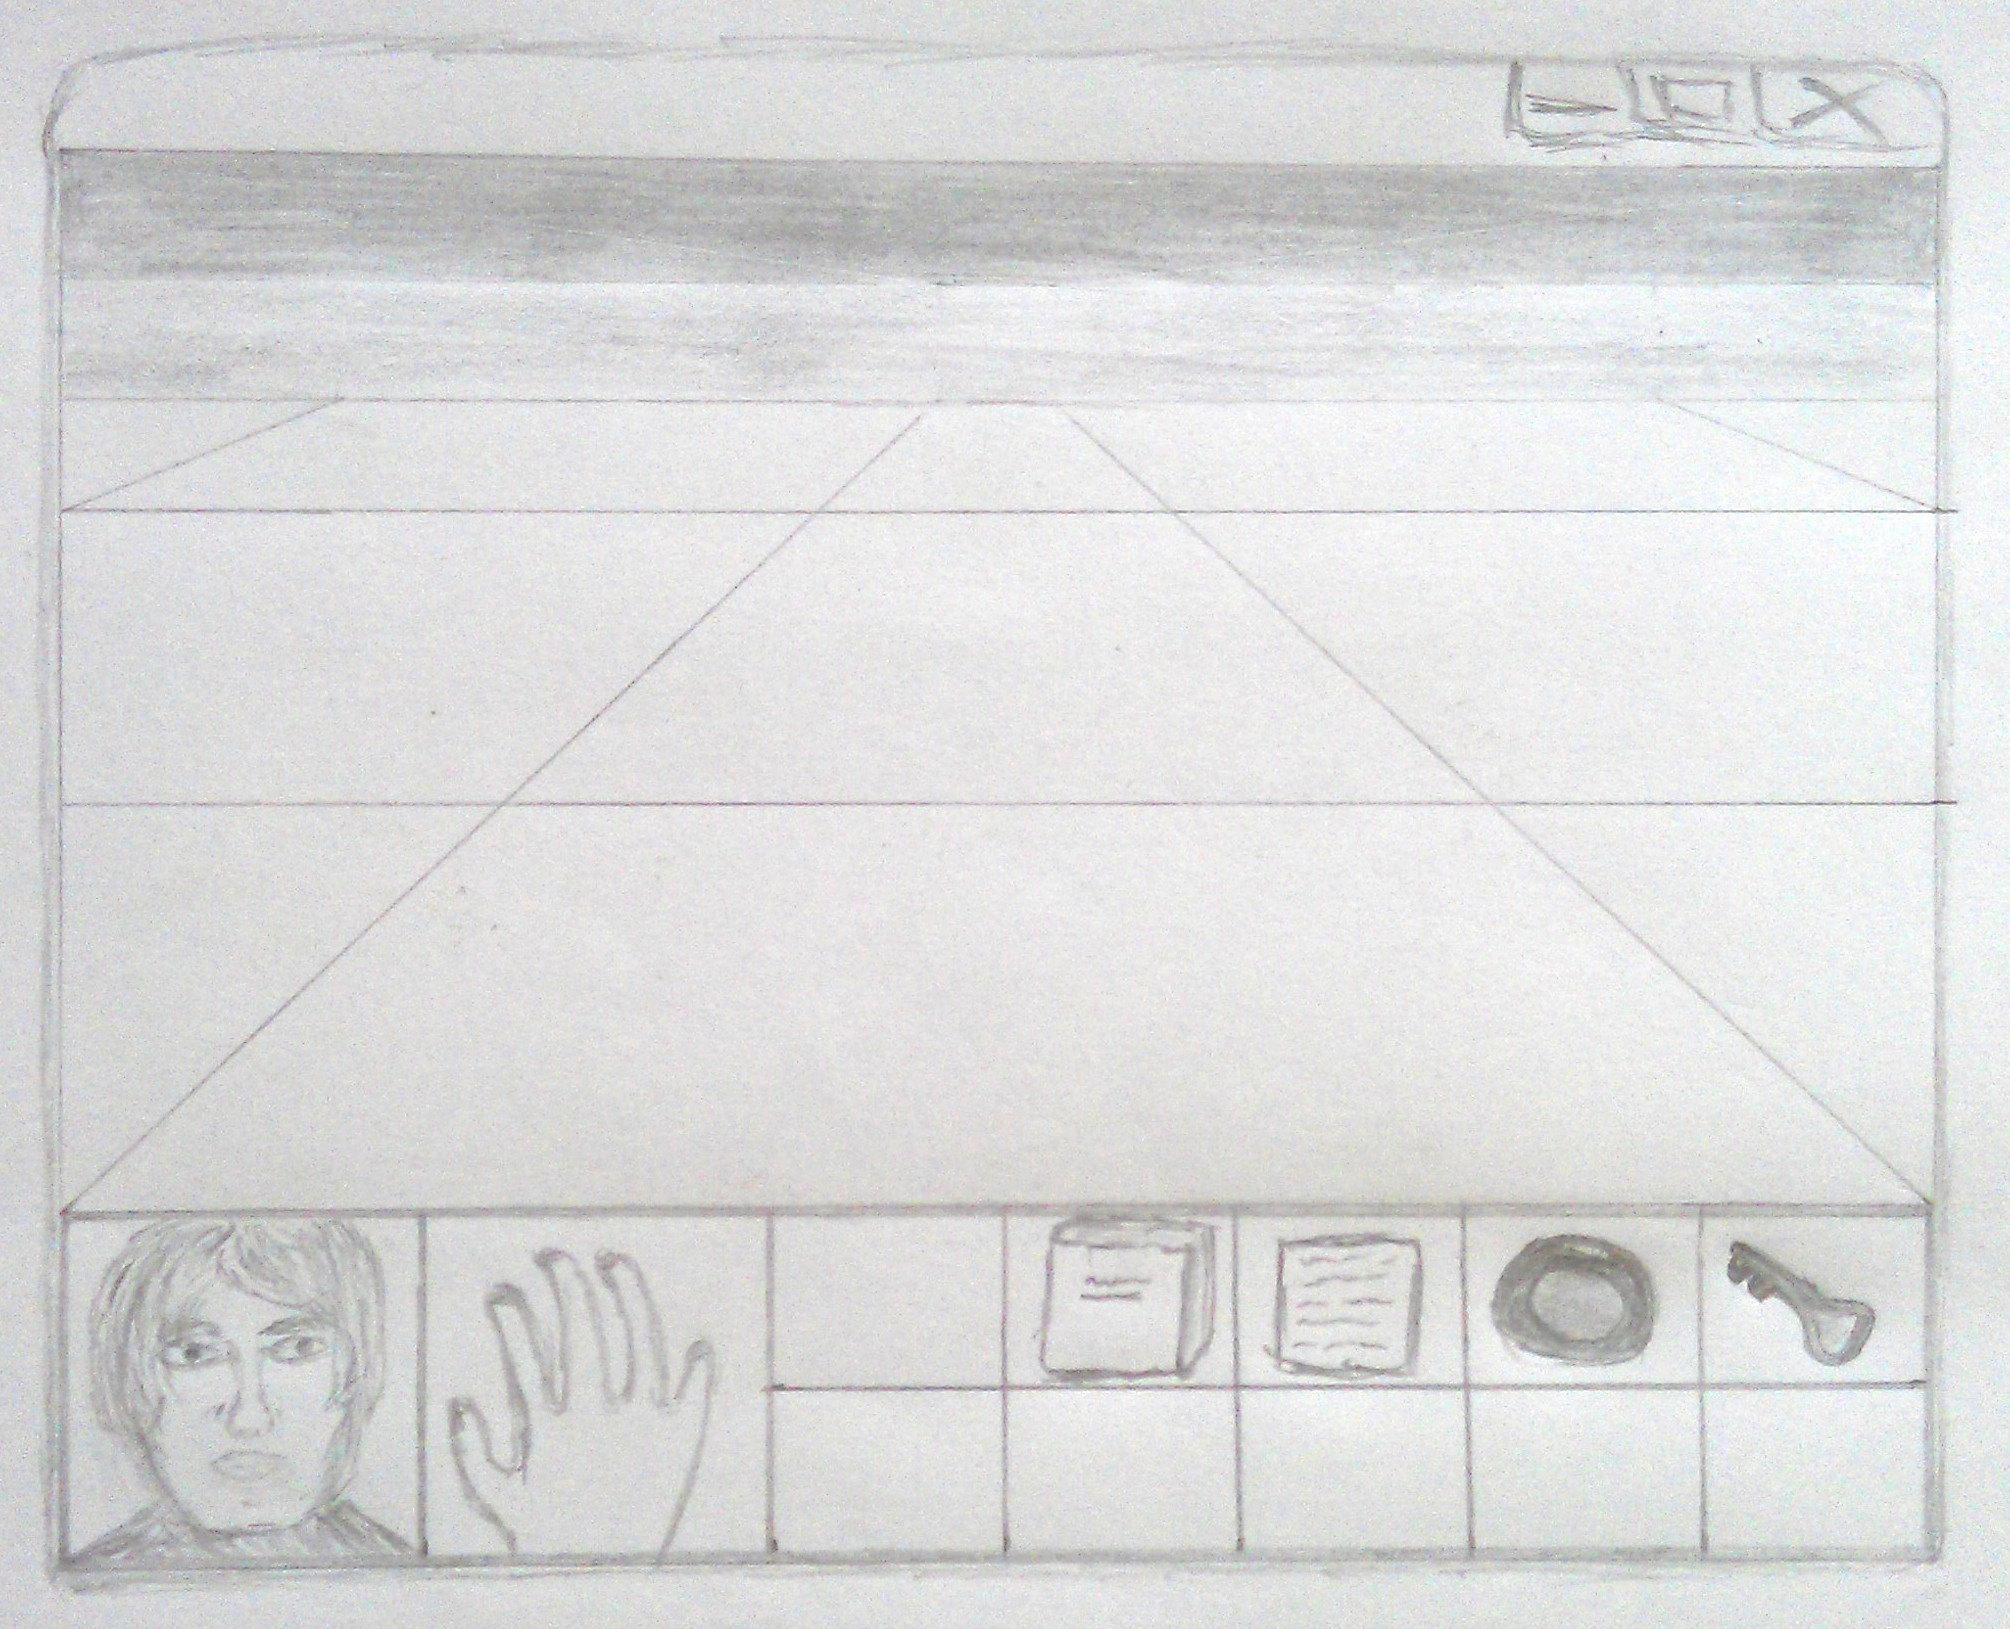
\includegraphics[width=13cm, height=10cm]{kapitel/ui/ig_leer_small.jpg}
	\end{center}
	\caption{Ein leerer Sichtbereich}
	\label{fig:ig_leer}
\end{figure}

Das Inventar in Abbildung \ref{fig:ig_leer} enthält einige Items, die der Nutzer bereits aufgesammelt hat.
Er hat aber kein Objekt in der Hand, daher die Darstellung der leeren Hand. Da er vor einem freien Bereich
steht, ist die Sichtweite am größten. Selbst in diesem Fall kann der Spieler aber nur drei Felder weit sehen
(das auf dem er sich momentan befindet eingeschlossen). Dahinter befinden sich eventuell weitere Felder, die
aber durch eine Art Nebel verhangen sind. Der Horizont ist also nicht sichtbar. Darüber befindet sich der
Himmel bzw. innerhalb von Gebäuden die Decke. 
\newpage
\begin{figure}[h]
	\begin{center}
		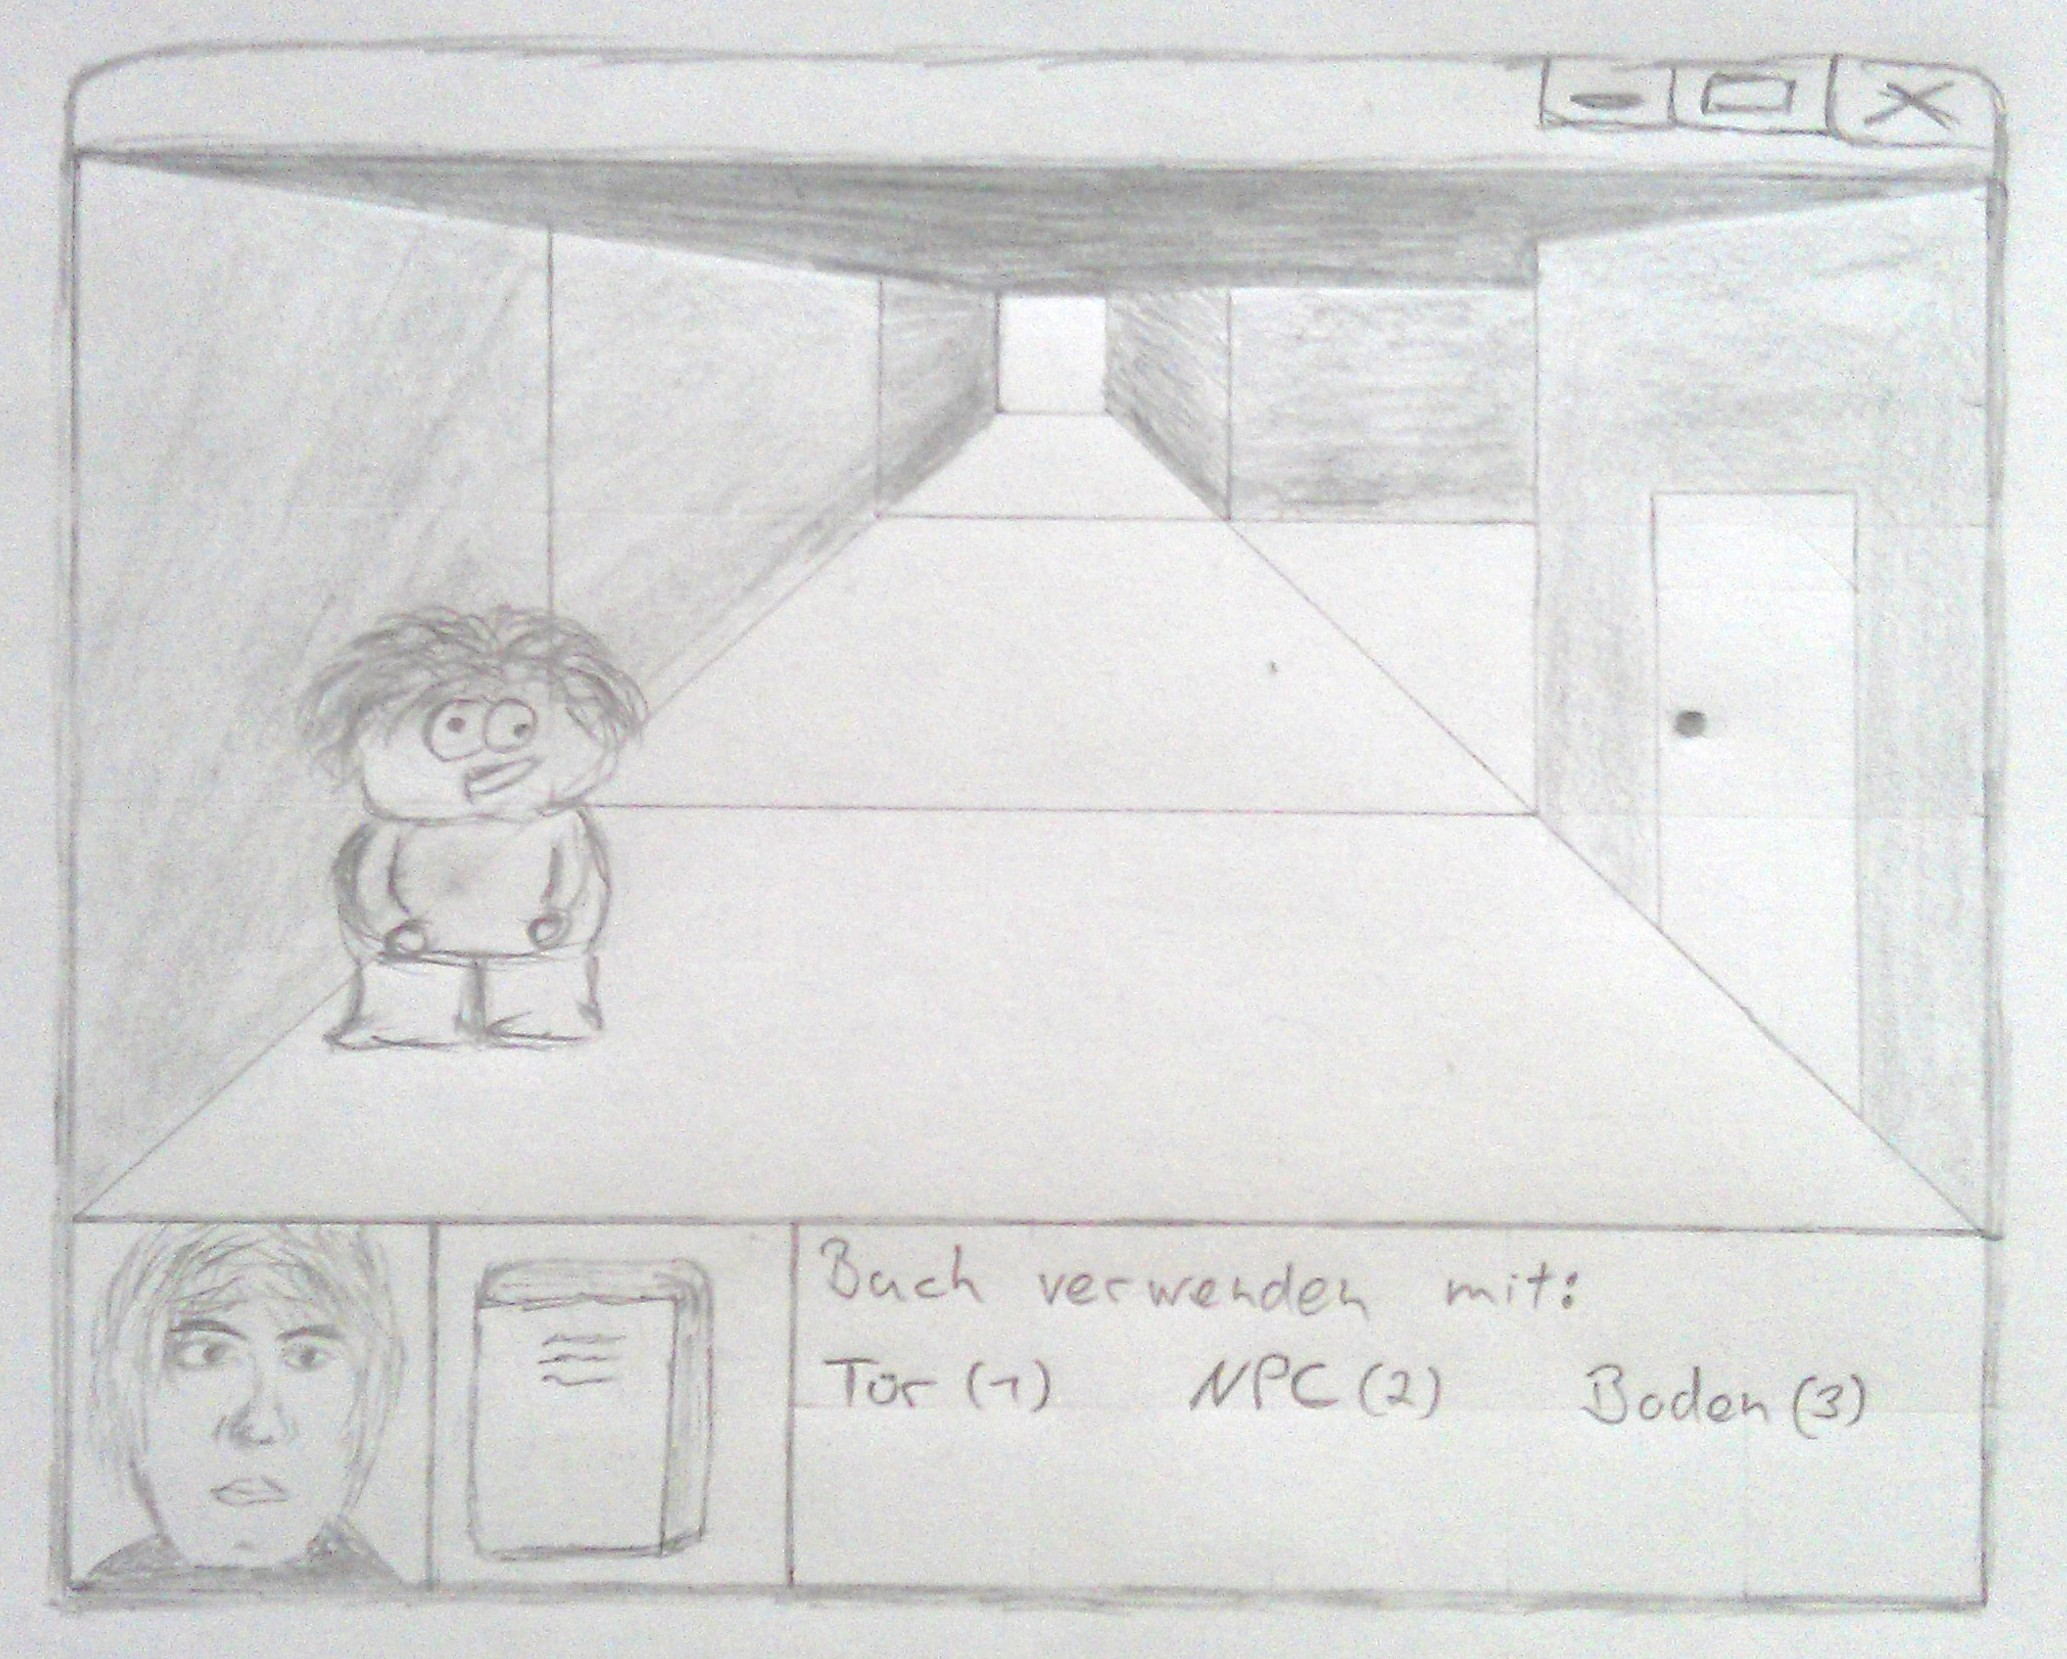
\includegraphics[width=13cm, height=10cm]{kapitel/ui/ig_npc_small.jpg}
	\end{center}
	\caption{Interaktion mit einem NPC}
	\label{fig:ig_npc}
\end{figure}
Abbildung \ref{fig:ig_npc} zeigt die Interaktion mit einem NPC. Der Infobereich zeigt jetzt textuelle
Informationen zur Interaktion an. Auch Dialoge werden in dieser Form dargestellt. Der Status- und Handbereich
bleiben in dieser Sicht erhalten, was praktisch ist um zum Beispiel eine Tür mit einem Schlüssel zu öffnen:
Man hat direkt im Blick, ob der Schlüssel schon in der Hand liegt, also verfügbar für diese Interaktion ist.
Wäre dies nicht der Fall, müsste dieser erst aus dem Inventar in die Hand genommen werden.
\newpage
\section{Menü GUI}
Die Menüs stellen die im Abschnitt 3 dargestellten Funktionen zur Verfügung. Wie dort angesprochen startet
der Spieler im Hauptmenü. Die Menüs sollen alle im gleichen Stil angelegt werden, daher werden hier nur zwei
Menüskizzen gezeigt. Die einzelnen Einträge können wie gesagt aus Abschnitt 3 übernommen werden.

\begin{figure}[htb]
	\begin{center}
		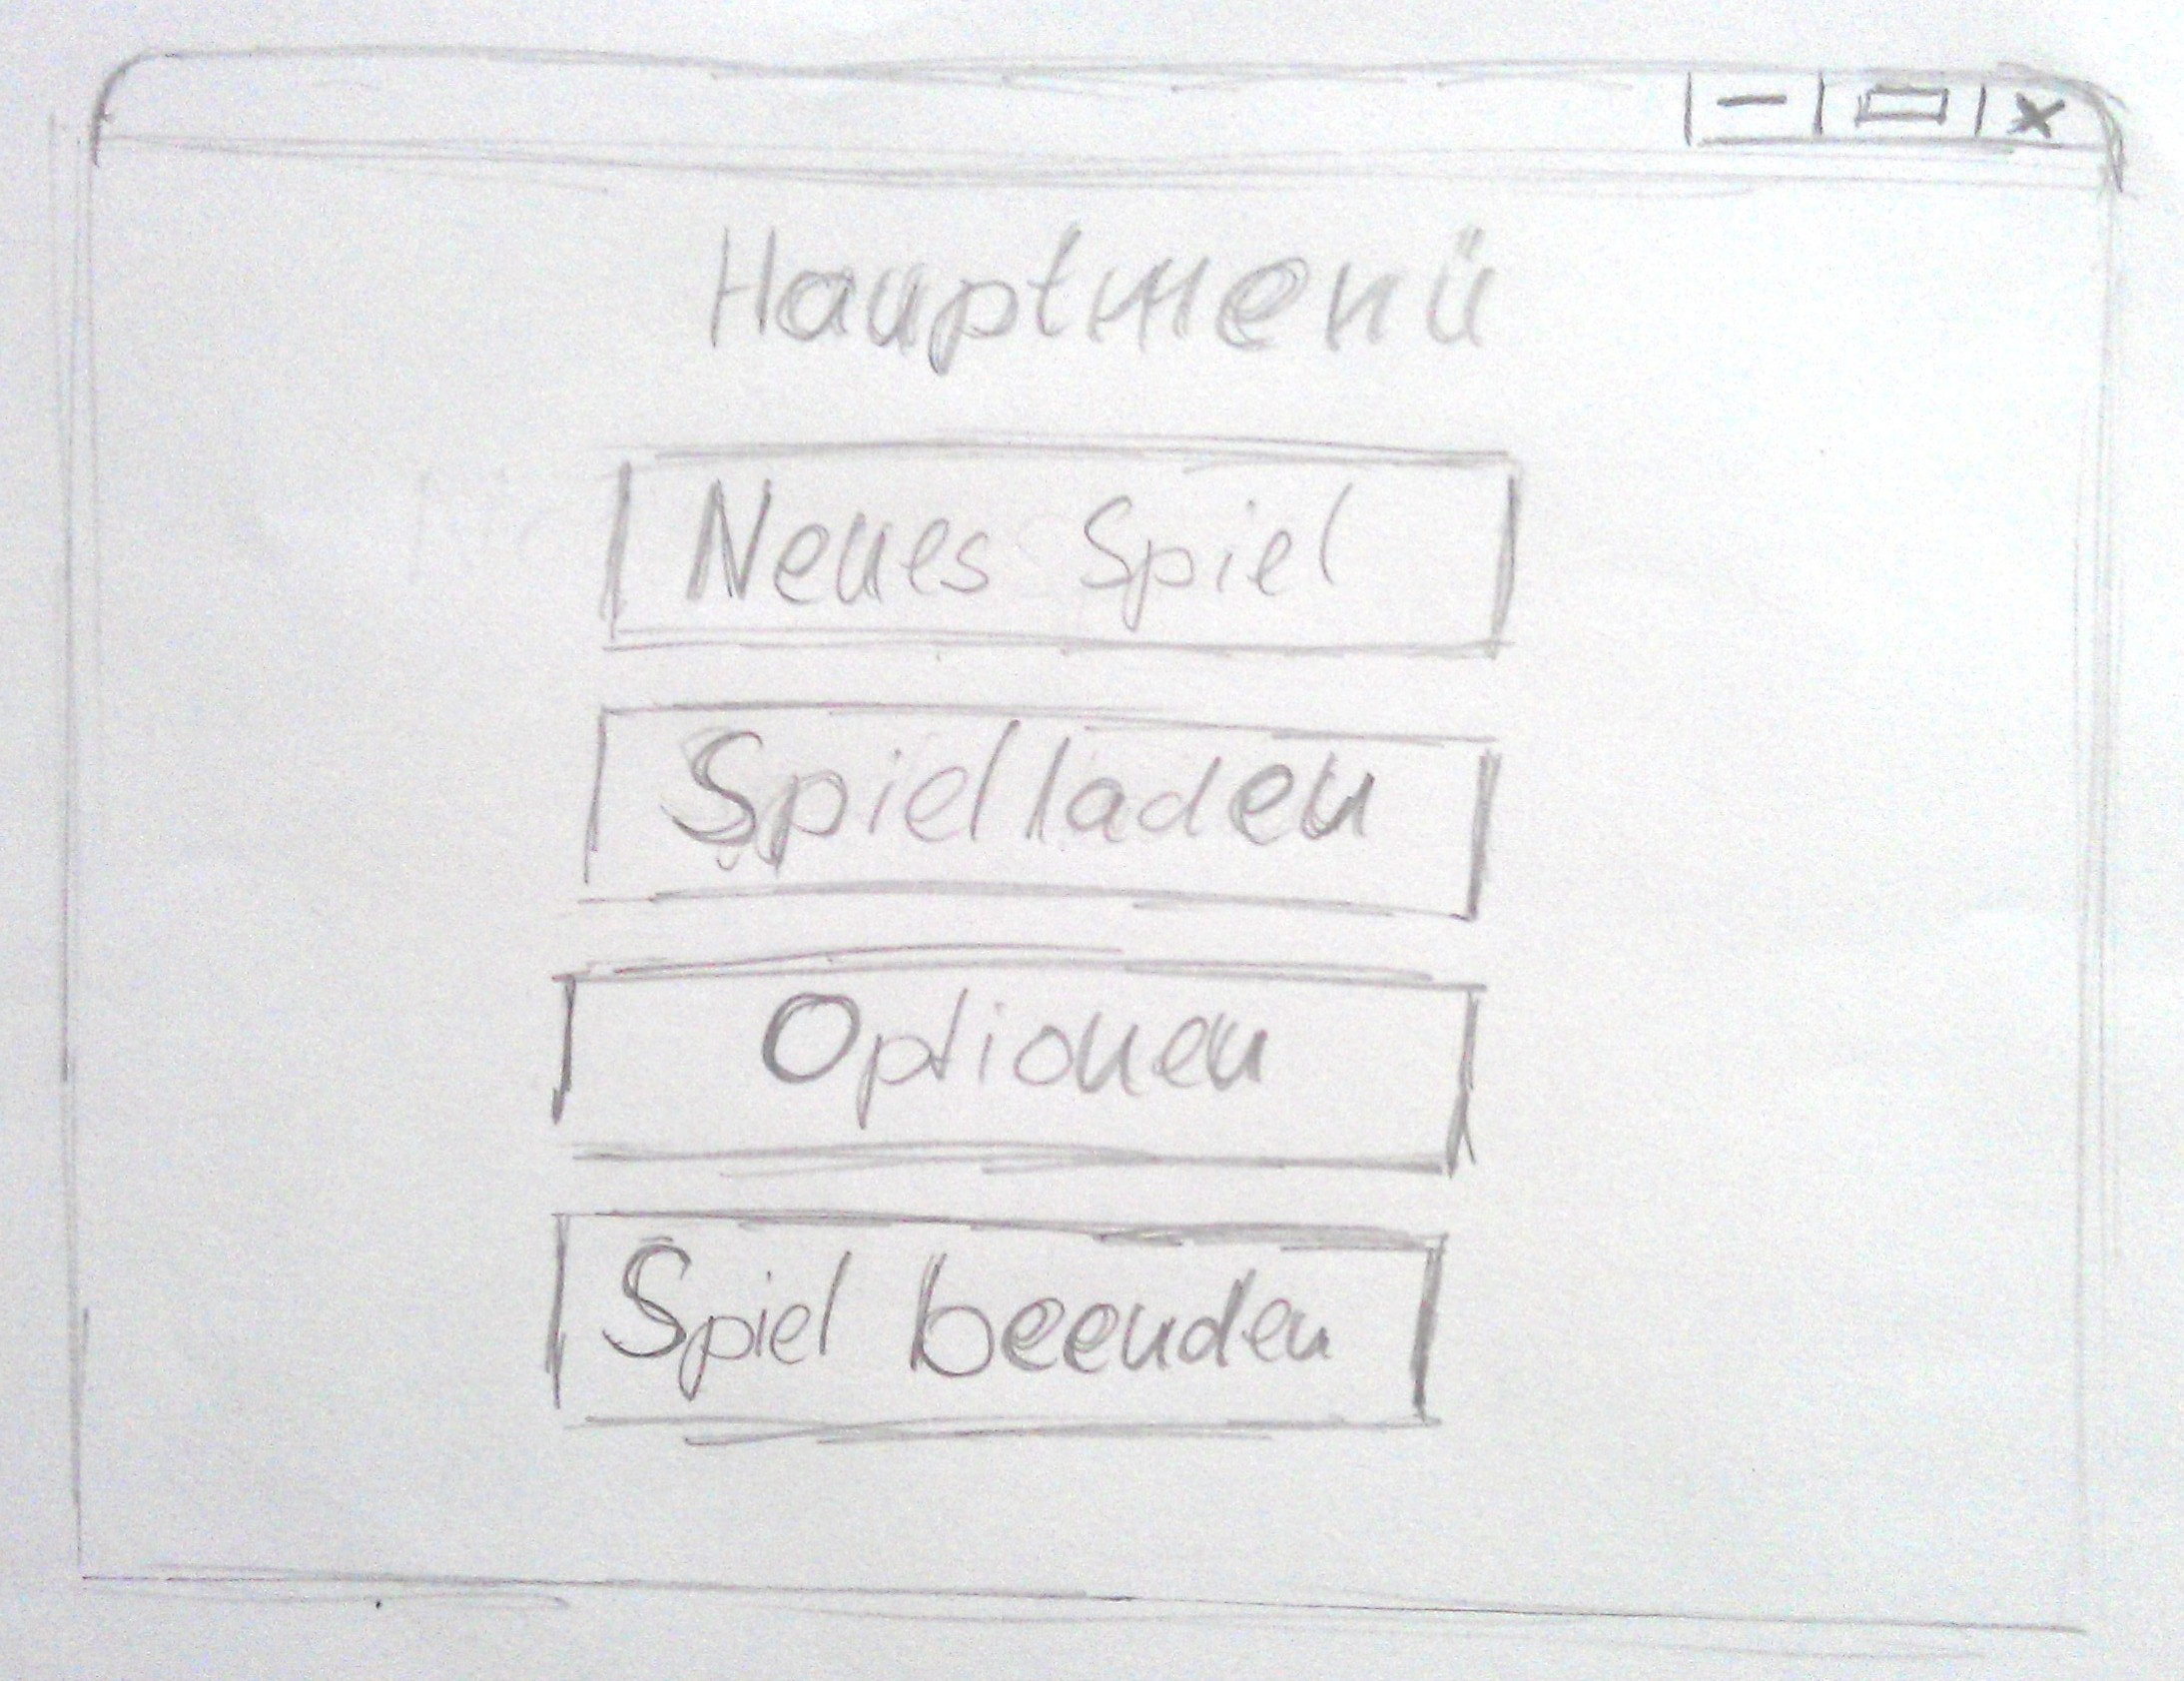
\includegraphics[width=9cm, height=6cm]{kapitel/ui/menu_main_small.jpg}
	\end{center}
	\caption{Das Hauptmenü}
	\label{fig:menu_main}
\end{figure}
Laden- und Speicherscreen wird es eine tabellarische Sicht mit den \glspl{Savegame} geben. Man hat jeweils
die Möglichkeit eines auszuwählen und zu laden bzw. ein neues anzulegen oder einzelne \glspl{Savegame} zu 
löschen.
\begin{figure}[htb]
	\begin{center}
		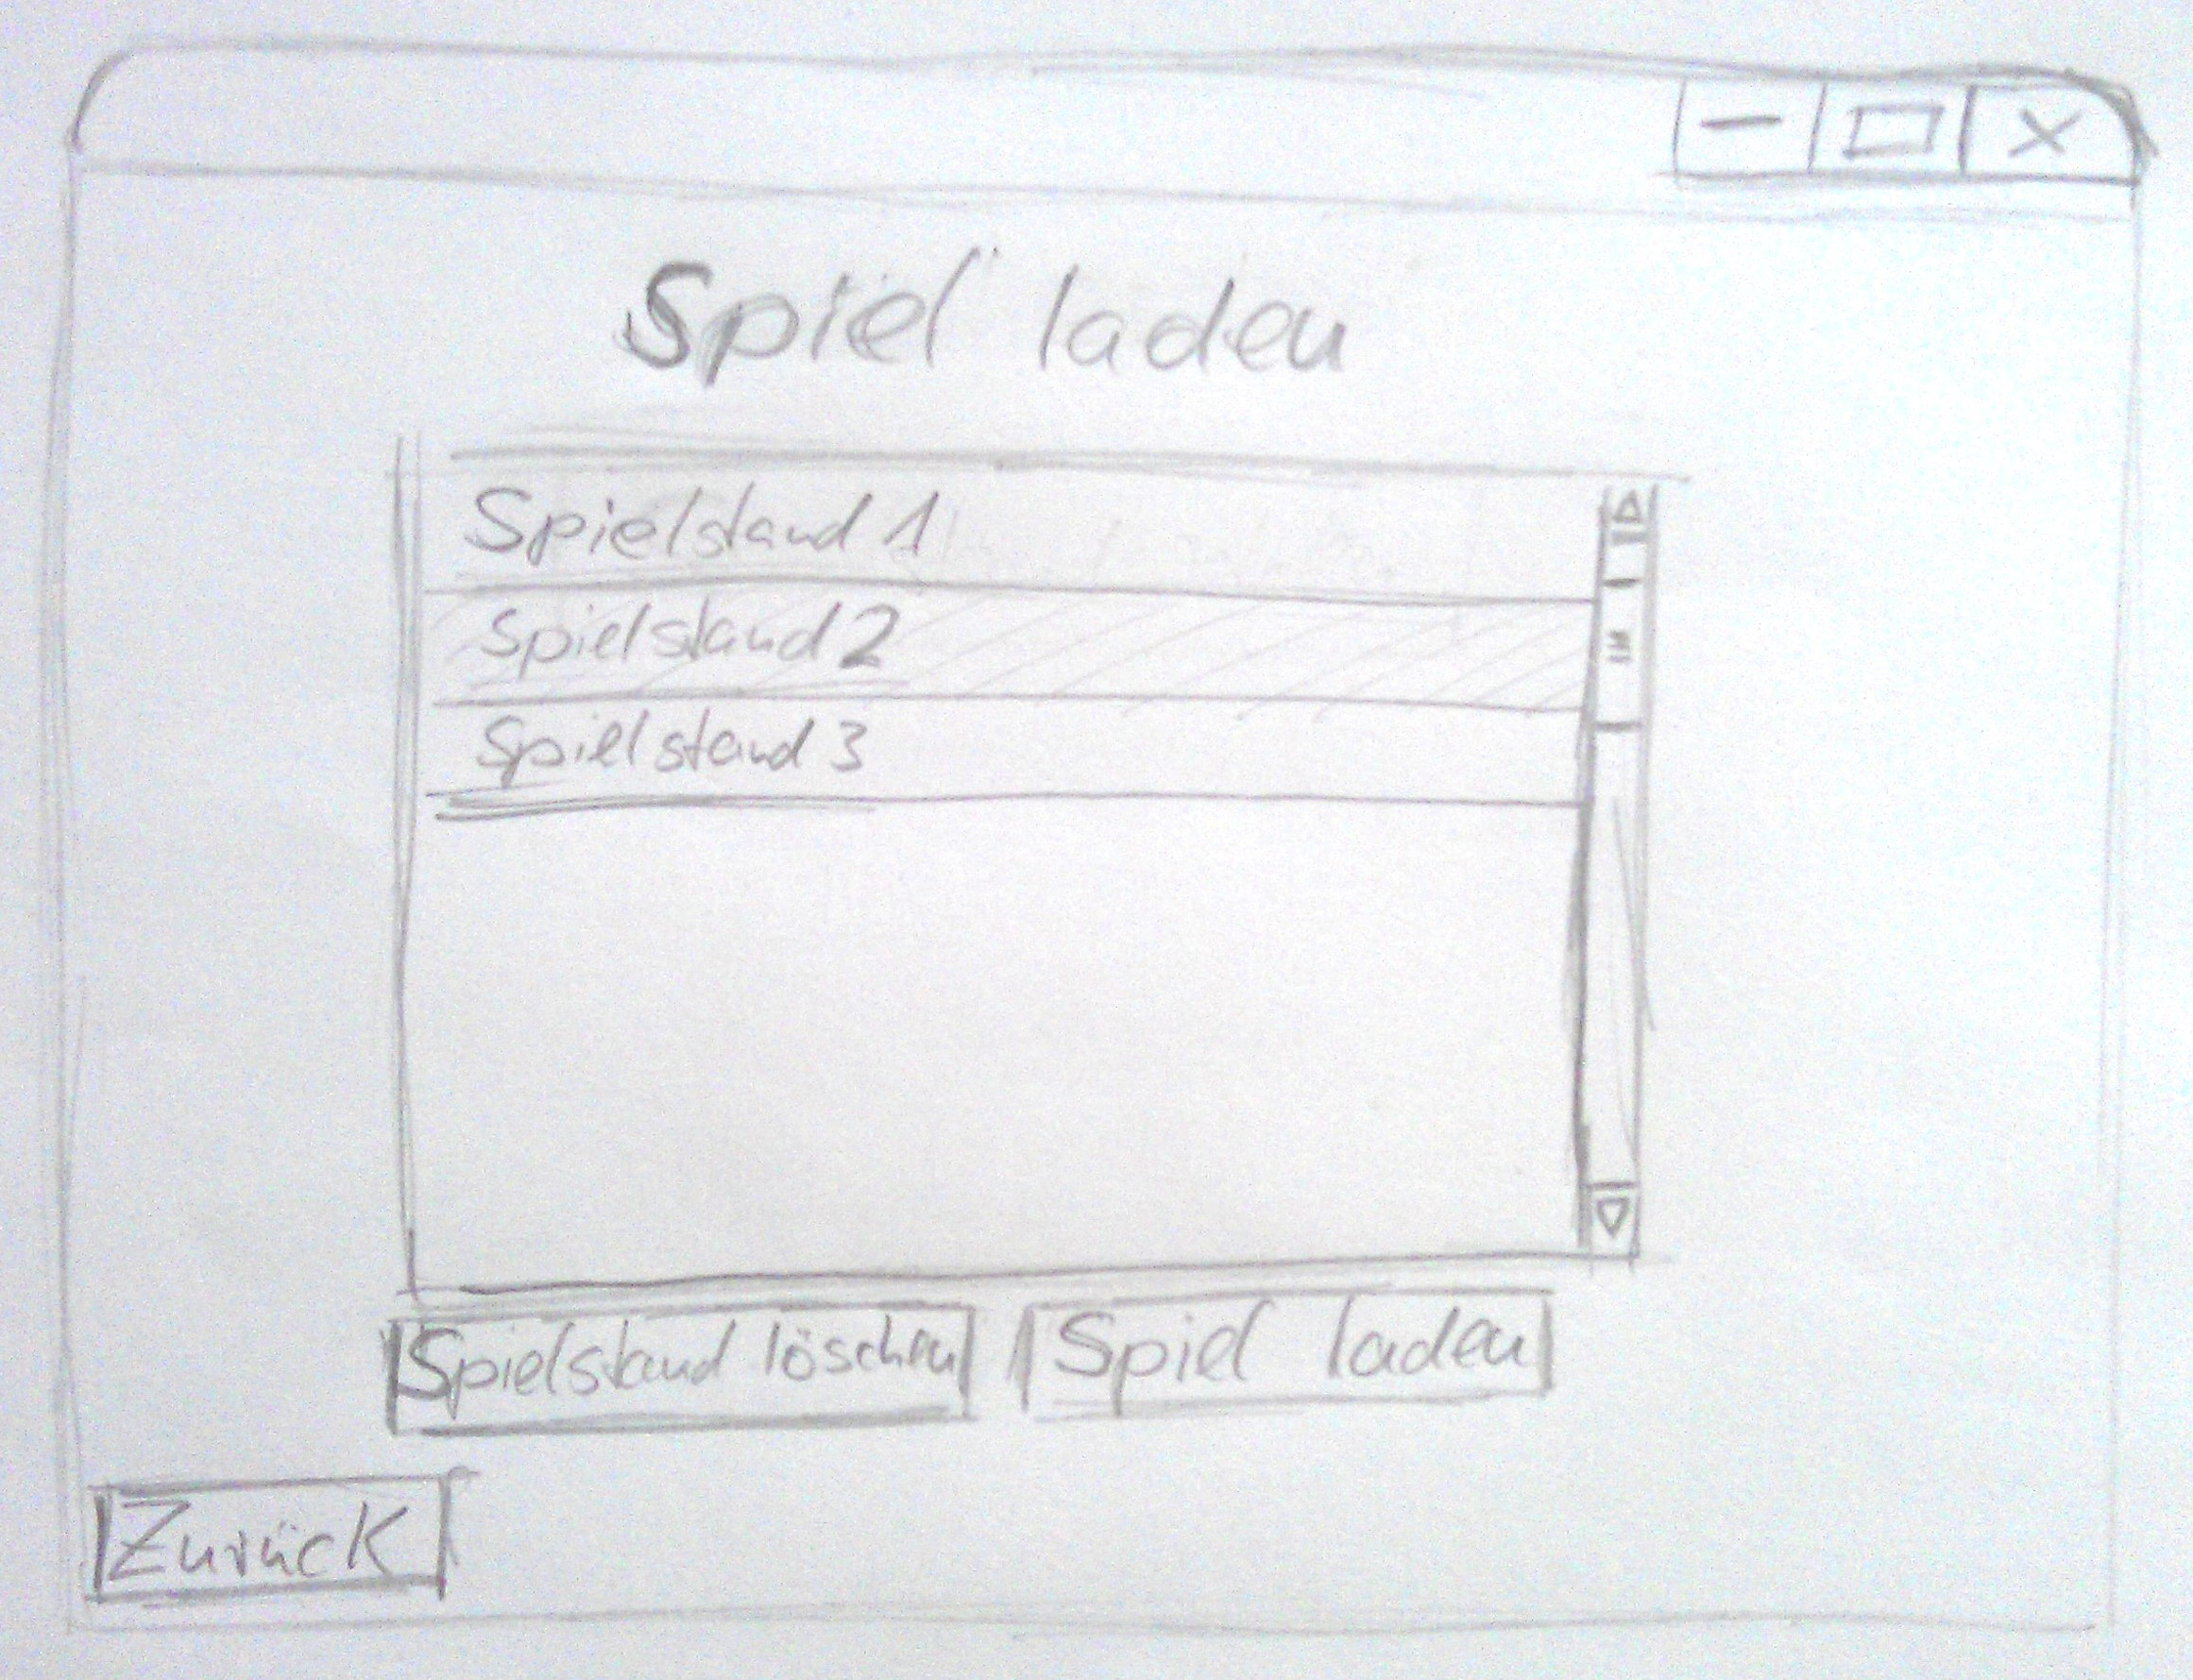
\includegraphics[width=9cm, height=6cm]{kapitel/ui/menu_load_small.jpg}
	\end{center}
	\caption{Das Lademenü}
	\label{fig:menu_load}
\end{figure}

\newpage
\section{Campusdatei \textit{(v0.1)}}
Die Campusdatei ist ein grundlegendes Konzept im Spiel, um den Campus konfigurierbar zu machen.
Dabei gibt es eine Standardvorgehensweise: Den Campus in Form von ASCII-Zeichen zu codieren
und dann die so entstandene Textdatei zu parsen. Da das Erstellen eines neuen Campus von Hand
so aber sehr umständlich werden kann (und Probleme mit der Positionierung auftreten könnten),
sollte der Campus als Bitmapdatei codiert werden. Letzten Endes ist auch eine Bitmap eine Textdatei
in der die Pixel Felder im Spiel darstellen und kann geparsed werden. Entscheidender Vorteil ist die 
bessere Les- und somit Benutzbarkeit.

\begin{figure}[h]
	\begin{center}
		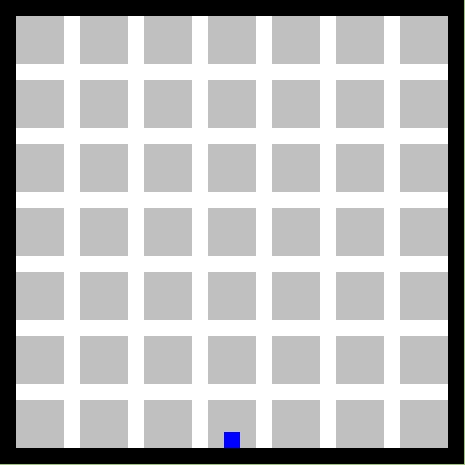
\includegraphics[width=7cm, height=7cm]{kapitel/ui/empty.png}
	\end{center}
	\caption{Ein leerer Campus}
	\label{fig:empty_campus}
\end{figure}

Das 29x29 Pixel große Minimalbeispiel einer solchen Datei wurde mit KolourPaint erstellt. Das Format der 
Datei ist PPM (Portable Pixel Map) in der Version P6 
(Spezifikation: \url{http://netpbm.sourceforge.net/doc/ppm.html}).
Die 3x3 großen Pixelfelder in Grau (\textit{0xC0C0C0}) stellen Felder auf dem Campus dar.
Die ein Pixel breiten Zwischenräume bieten Platz für Wände (\textit{0x000000}) und Türen (grün 
\textit{0x00FF00} oder rot \textit{0xFF0000}). Die Starposition des Spielers
wird durch einen blaues (\textit{0x0000FF}) Pixel innerhalb eines Feldes verdeutlicht. 

\begin{figure}[h]
	\begin{center}
		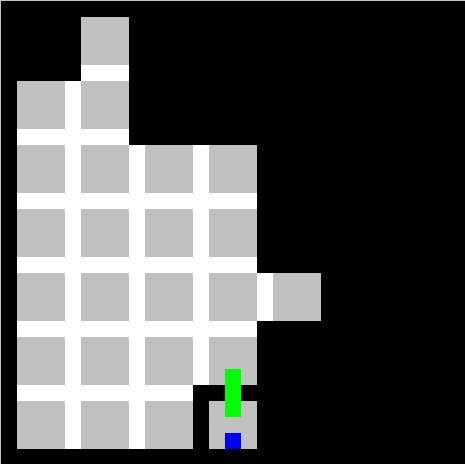
\includegraphics[width=7cm, height=7cm]{kapitel/ui/room_door_fancy.png}
	\end{center}
	\caption{Zwei Räume mit Tür}
	\label{fig:room_door_fancy}
\end{figure}

Es soll nicht möglich sein, Wände quer über ein Feld zu zeichnen. Allein die Zwischenräume bieten Platz für
Wanddefinitionen. Sollen Felder untereinander frei zugänglich sein, so bleibt der Zwischenraum weiss 
(\textit{0xFFFFFF}). Sollen Felder zwar durch eine Wand getrennt, aber mittels einer Tür verbunden sein,
so wird dies durch ein grünes (\textit{0x00FF00}) Pixel im Fall einer offenen, oder ein rotes 
(\textit{0xFF0000}) Pixel im Fall einer verschlossenen Tür dargestellt. Türen und Wände sind die einzigen
Gegenstände die im Zwischenraum positioniert werden dürfen. Türen belegen zusätzlich auf den Feldern die sie
verbinden einen Slot (in der gleichen Farbe die die jeweilige Tür markiert). Zu beachten ist auch, dass der
auf diese Art und Weise gezeichnete Campus immer einen ein Pixel großen Rand hat (\textit{0x000000} oder
\textit{0xFFFFFF}) und die Felder nur immer jeweils um drei Pixel gegeinander verschoben werden können, die
Feldkanten sind also immer bündig zu einander angelegt. Das gleiche gilt für Wände. Ein Feld ist immer 3x3
Pixel groß, ein Wandstück immer 3x1 Pixel lang. Es können allerdings mehrere dieser Wandteile aneinander
gefügt werden, wie in Abbildung \ref{fig:room_door_fancy} zu sehen, falls größere Bereiche zum Beispiel nicht
begehbar sein sollen.

Die Mapdatei muss eine Versionsnummer haben. Da die Versionsnummer für unser Spiel im PPM Format nicht 
vorgesehen ist, muss jede Mapdatei als Dateiendung "ctfmap\textit{xx}" haben. Die Nummer \textit{xx} ist die 
zugehörige Versionsnummer des Spiels (ohne trennenden Punkt) und die Campusdatei ist genau für diese Version
zulässig. Je nach Version können weitere Objekte auf
den Feldern der Map positioniert werden, Grundlage ist aber immer die Version 0.1. Die angegebenen Pixelgrößen
gehören zum definierten Campusformat dazu und müssen immer berücksichtigt werden. Dateien, die nicht genau das
angegebene Format haben, können nicht eingelesen werden.
